\chapter{Hasil dan Pembahasan}

Bab ini menyajikan hasil dan analisis mendalam terhadap sistem RAG berbasis \textit{Knowledge Graph} yang telah dirancang dan diimplementasikan.
Penyajian dimulai dari tahap \textit{knowledge extraction} dari korpus dokumen.
Selanjutnya dipaparkan hasil evaluasi kuantitatif dari rancangan arsitektur RAG baik pada komponen \textit{retriever} maupun jawaban final yang dihasilkan oleh sistem secara keseluruhan.
Setiap hasil akan diikuti dengan pembahasan untuk menginterpretasikan data, menganalisis kekuatan dan kelemahan sistem, serta menyajikan studi kasus untuk memberikan gambaran yang lebih jelas.

\section{Hasil \textit{Knowledge Extraction}}
Proses \textit{knowledge extraction} dimulai dengan ekstraksi teks dari dokumen.
Dokumen yang dalam format HTML atau DOCX kemudian diambil teks yang terkandung di dalamnya sekaligus dilakukan \textit{structural chunking} untuk membaginya ke dalam beberapa potongan berdasarkan tingkatan hierarki tertentu.
Proses \textit{chunking} hanya dilakukan pada dokumen buku "Petunjuk Teknis Pencegahan dan Pengendalian Gangguan Mental Emosional" karena berukuran cukup besar yaitu sekitar 15.000 kata dibandingkan dengan dokumen lainnya yang kurang dari 6.000 kata.
Hal tersebut dilakukan mengingat LLM kesulitan untuk secara detail memahami isi dari dokumen tersebut.
Dari proses \textit{chunking} tersebut menghasilkan total 17 potongan dokumen yang disimpan dalam format TXT.

Sejumlah 17 potongan dokumen tersebut kemudian dimasukkan ke dalam LLM untuk diekstrak entitas dan relasi secara berurutan.
Dari proses ekstraksi tersebut menghasilkan 1.119 entitas dan 1.078 relasi secara keseluruhan.
Tabel \ref{tab:knowledge-graph-stats} menunjukkan statistik \textit{Knowledge Graph} yang dihasilkan dari dokumen secara keseluruhan

\begin{table}[h]
	\centering
	\caption{Statistik \textit{Knowledge Graph} yang dihasilkan dari dokumen}
	\label{tab:knowledge-graph-stats}
	{\setlength{\tabcolsep}{0.5em}
		\begin{tabular}{|l|r|}
			\hline
			\textbf{Komponen}         & \textbf{Jumlah} \\
			\hline \hline
			\textbf{Dokumen}          &
			5                                           \\
			\hline
			\textbf{Potongan Dokumen} &
			17                                          \\
			\hline
			\textbf{Entitas}          &
			1119                                        \\
			\hline
			\textbf{Relasi}           &
			1073                                        \\
			\hline
			\textbf{Jenis Entitas}    &
			18                                          \\
			\hline
			\textbf{Jenis Relasi}     &
			18                                          \\
			\hline
		\end{tabular}}
\end{table}


Suatu fakta yang berhasil diekstrak dari dokumen akan disimpan dalam bentuk triplet (subjek, predikat, dan objek), yang kemudian diimplementasikan sebagai \textit{node} dan \textit{edge} dalam struktur graf pengetahuan.
Sebagai contoh, berikut adalah sebuah potongan dokumen yang dianalisis:

\begin{quote}
	\itshape
	Faktor psikologis yaitu kegagalan, kekecewaan, trauma yang mengakibatkan stres dan faktor biologis yaitu genetik, gizi dan infeksi perinatal serta kondisi lingkungan yang buruk juga merupakan faktor yang berkontribusi terhadap terjadinya gangguan jiwa.

	\textbf{Faktor Psikologis} \\
	Faktor psikologis yang menjadi faktor risiko GME, antara lain (Kerig, Ludlow, \& Wenar, 2012; PPSDM Kemenkes RI, 2016):
	\begin{enumerate}
		\item Regulasi emosi rendah
		\item Kemampuan regulasi diri rendah yang termanifestasikan dalam kontrol perilaku yang buruk
		\item Konsep diri negatif
		\item Efikasi diri rendah
		\item Resiliensi diri rendah
	\end{enumerate}

	\textbf{Cara menangani Resiliensi Diri Rendah:}
	\begin{enumerate}[label=\alph*)]
		\item Melatih keterampilan manajemen stres
		\item Melatih fleksibilitas dalam berpikir dan keterampilan pengambilan keputusan
		\item Melatih keterampilan manajemen konflik
	\end{enumerate}
	\normalfont
\end{quote}

Berdasarkan potongan dokumen tersebut, sistem ekstraksi menghasilkan beberapa triplet pengetahuan sebagai berikut:

\begin{lstlisting}[frame=single, numbers=none, basicstyle=\ttfamily\footnotesize]
(:Gangguan_Mental {name: "Gangguan Jiwa"})<-[:Berkontribusi_Pada]-(:Faktor_Risiko {name: "Faktor Psikologis"})

(:Gangguan_Mental {name: "Gangguan Jiwa"})<-[:Berkontribusi_Pada]-(:Faktor_Risiko {name: "Faktor Biologis"})

(:Gejala {name: "Resiliensi Diri Rendah"})-[:Adalah_Jenis_Dari]->(:Faktor_Risiko {name: "Faktor Psikologis"})

(:Aktivitas_Kesejahteraan {name: "Manajemen Konflik"})-[:Menangani]->(:Gejala {name: "Resiliensi Diri Rendah"})

(:Aktivitas_Kesejahteraan {name: "Keterampilan Pengambilan Keputusan"})-[:Menangani]->(:Gejala {name: "Resiliensi Diri Rendah"})
\end{lstlisting}

\section{Hasil Pengembangan Arsitektur RAG Berbasis \textit{Knowledge Graph}}

Sistem yang dikembangkan berupa AI \textit{service} berbasis arsitektur RAG dengan \textit{Knowledge Graph}.
Layanan AI tersebut disediakan dalam bentuk REST API sehingga memudahkan dalam integrasi dengan platform lain.
Antarmuka aplikasi REST juga memudahkan dalam pengujian dan menyimulasikan sistem ketika diimplementasikan pada skenario penggunaan sebenarnya.
Arsitektur dirancang untuk mendukung proses penjawaban pertanyaan yang memprioritaskan jawaban berbasis konteks.
Basis konteks tersebut diperoleh dari pengambilan informasi pada \textit{Knowledge Graph} dengan memanfaatkan entitas dan relasi yang terkandung di dalamnya.
AI \textit{service} dapat diakses melalui HTTP \textit{request} dengan spesifikasi seperti pada Tabel \ref{tab:ai-service-answer}.

\begin{longtable}{|p{0.3\textwidth}|p{0.65\textwidth}|}
	\caption{Spesifikasi \textit{endpoint} untuk menghasilkan jawaban}
	\label{tab:ai-service-answer}                                                               \\
	\hline
	\textbf{Komponen}             & \textbf{Nilai}                                              \\
	\hline \hline
	\endfirsthead

	\hline
	\textbf{Komponen}             & \textbf{Nilai}                                              \\
	\hline \hline
	\endhead


	\textbf{URL}                  &
	http://localhost:8080/api/v1/retrieval/get-answer                                           \\
	\hline
	\textbf{HTTP \textit{Method}} &
	POST                                                                                        \\
	\hline
	\textbf{\textit{Body} (JSON)} & \begin{lstlisting}[basicstyle=\ttfamily\small, numbers=none]
{
  "query": "",
  "graph_traversal": "",
  "search_method": "",
  "max_hop": 0,
  "limit": 0,
  "top_k": 0
}
    \end{lstlisting} \\
	\hline
	\textbf{Respons (JSON)}       & \begin{lstlisting}[basicstyle=\ttfamily\small, numbers=none]
{
  "message": "",
  "data": {
    "latency" : 0.0,
    "method": "",
    "query_class": {
      "category": "",
      "entities": []
    },
    "answer" : "",
    "knowledge": "",
    "graph" : {}
  }
}
    \end{lstlisting} \\
	\hline
\end{longtable}

Untuk memperoleh respons dari sistem dilakukan pemanggilan API dengan spesifikasi seperti pada Tabel \ref{tab:ai-service-answer}.
Berikut merupakan potongan contoh respons sistem untuk pertanyaan \textit{"Apa itu Gangguan Mental Emosional?"} pada Tabel \ref{tab:ai-service-response-example}.

\begin{longtable}{|p{0.2\textwidth}|p{0.7\textwidth}|}
	\caption{Contoh respons sistem dalam menghasilkan jawaban}
	\label{tab:ai-service-response-example}                                                    \\
	\hline
	\textbf{Komponen}            & \textbf{Isi}                                                \\
	\hline \hline
	\endfirsthead

	\hline
	\textbf{Komponen}            & \textbf{Isi}                                                \\
	\hline \hline
	\endhead


	Kueri                        &
	Apa itu Gangguan Mental Emosional?                                                         \\
	\hline
	\textit{Request Body}        & \begin{lstlisting}[basicstyle=\ttfamily\small, numbers=none]
{
  "query": "Apa itu Gangguan Mental Emosional?",
  "graph_traversal": "auto",
  "search_method": "auto",
  "max_hop": 10,
  "limit": 50,
  "top_k": 3
}
    \end{lstlisting} \\
	\hline
	Konteks \newline Pengetahuan &
	Berikut adalah informasi yang ditemukan dari knowledge graph:

	\textbf{Entitas: Gangguan Mental Emosional} (Tipe: Gangguan\_Mental)
	\begin{itemize}
		\item Deskripsi: Bukan diagnosis gangguan jiwa.
		      Dapat memengaruhi aktifitas sehari-hari yang berdampak pada menurunnya produktifitas dan kualitas hidup.
		      Kondisi atau gangguan yang menjadi subjek utama dari 'Petunjuk Teknis Pencegahan dan Pengendalian Gangguan Mental Emosional'.
		      ....
		\item Skor Relevansi Awal: 5.07
		\item Hubungan Terkait:
		      \begin{itemize}
			      \item[$\rightarrow$] \textsl{merupakan} $\rightarrow$ Masalah Kesehatan Jiwa
			      \item[$\rightarrow$] \textsl{mengindikasikan} $\rightarrow$ Perubahan Psikologis
			      \item[$\leftarrow$] \textsl{mencegah} $\leftarrow$ Upaya Promosi Kesehatan
			      \item [...]
		      \end{itemize}
	\end{itemize}
	\textbf{Entitas: Deteksi Gangguan Mental Emosional} (Tipe: Layanan\_Kesehatan)
	\begin{itemize}
		\item Deskripsi: Proses identifikasi gangguan mental emosional yang diharapkan mampu dilakukan oleh fasilitas pelayanan kesehatan primer.
		\item Skor Relevansi Awal: 4.52
		\item Hubungan Terkait:
		      \begin{itemize}
			      \item[$\leftarrow$] \textsl{mampu melakukan} $\leftarrow$ Fasilitas pelayanan kesehatan primer
			      \item[$\rightarrow$] \textsl{dapat segera diintervensi} $\rightarrow$ Intervensi
			      \item[...]
		      \end{itemize}
	\end{itemize}
	\textbf{Penderita Gangguan Mental Emosional} (Tipe: Individu)
	\begin{itemize}
		\item Deskripsi: Proses identifikasi gangguan mental emosional yang diharapkan mampu dilakukan oleh fasilitas pelayanan kesehatan primer.
		      ... (Informasi selengkapnya dapat dilihat pada Lampiran)
	\end{itemize}
	\\
	\hline

	Jawaban                      &
	Gangguan Mental Emosional (GME) adalah suatu kondisi yang mengindikasikan seseorang mengalami perubahan psikologis. Perubahan ini bisa merupakan kondisi normal, namun dapat juga merupakan kondisi patologis.

	Penting untuk diketahui bahwa Gangguan Mental Emosional \textbf{bukanlah diagnosis gangguan jiwa}. Meskipun demikian, kondisi ini merupakan masalah kesehatan jiwa yang banyak dijumpai di Indonesia, diperkirakan diderita oleh 19 juta orang.

	GME dapat memengaruhi aktivitas sehari-hari seseorang, yang pada akhirnya berdampak pada menurunnya produktivitas dan kualitas hidup. Istilah ini juga digunakan dalam ``Petunjuk Teknis Pencegahan dan Pengendalian Gangguan Mental Emosional'' sebagai subjek utama panduan tersebut.
	\\
	\hline
\end{longtable}

Pada potongan contoh respons sistem untuk pertanyaan \textit{"Apa itu Gangguan Mental Emosional"} pada tabel \ref{tab:ai-service-response-example}, sistem akan mengambil konteks pengetahuan yang diperoleh dari \textit{Knowledge Graph}.
Terlihat dalam konteks pengetahuan yang diambil sistem berhasil mengambil beberapa entitas utama (Gangguan Mental Emosional, Deteksi Gangguan Mental Emosional, dan Penderita Gangguan Mental Emosional) beserta entitas tetangganya.
Konteks pengetahuan yang diperoleh tidak hanya menyediakan definisi, tetapi juga relasi antar entitas, seperti "merupakan", "mengindikasikan", dan "mencegah".
Hal tersebut sangat penting untuk menyediakan konteks bagi LLM sehingga mampu menghasilkan jawaban yang holistik.
Jawaban yang dihasilkan tidak hanya menjawab pertanyaan \textit{"Apa itu Gangguan Mental Emosional?"} secara langsung, tetapi juga memberikan informasi tambahan yang relevan dan penting.
Jawaban akhir secara langsung merefleksikan dan menyintesis informasi yang ada di dalam konteks pengetahuan, membuktikan bahwa sistem tidak berhalusinasi, setidaknya pada contoh ini.

\section{Hasil Pengembangan \textit{Dataset} Evaluasi Sitetis}
\textit{Dataset} evaluasi diperoleh secara sintesis melalui proses \textit{prompting} pada model OpenAI o4-mini.
Data yang dihasilkan berupa pasangan \textit{query} atau pertanyaan dan \textit{golden aswer} atau jawaban yang dianggap sebagai acuan jawaban yang diharapkan.
Selain itu dibubuhkan juga \textit{golden nodes} yang merujuk pada \textit{nodes} yang relevan untuk menjawab pertanyaan dan \texttt{query\_lable} untuk menandai jenis pertanyaan.
Dari proses \textit{prompting} diperoleh hasil berupa 433 data evaluasi yang terdiri dari 266 \texttt{entity\_query} dan 167 \texttt{path\_query} seperti pada Tabel \ref{tab:evaluation-dataset-result}.
Setiap pertanyaan tersebut dijamin memiliki referensi ke setidaknya satu \textit{node} dalam \textit{Knowledge Graph}.
Contoh dataset sintesis yang dihasilkan dapat dilihat pada Gambar \ref{fig:evaluation-dataset-example}.

\begin{table}[H]
	\centering
	\caption{Hasil sintesis \textit{dataset} evaluasi menggunakan model OpenAI o4-mini}
	\label{tab:evaluation-dataset-result}
	\begin{tabular}{|l|r|}
		\hline
		\textbf{Kategori Kueri} & \textbf{Jumlah} \\
		\hline \hline
		\texttt{entity\_query}  &
		266                                       \\
		\hline
		\texttt{path\_query}    &
		167                                       \\
		\hline
		\textbf{Total}          &
		433                                       \\
		\hline
	\end{tabular}
\end{table}


\begin{figure}[H]
	\centering
	\fbox{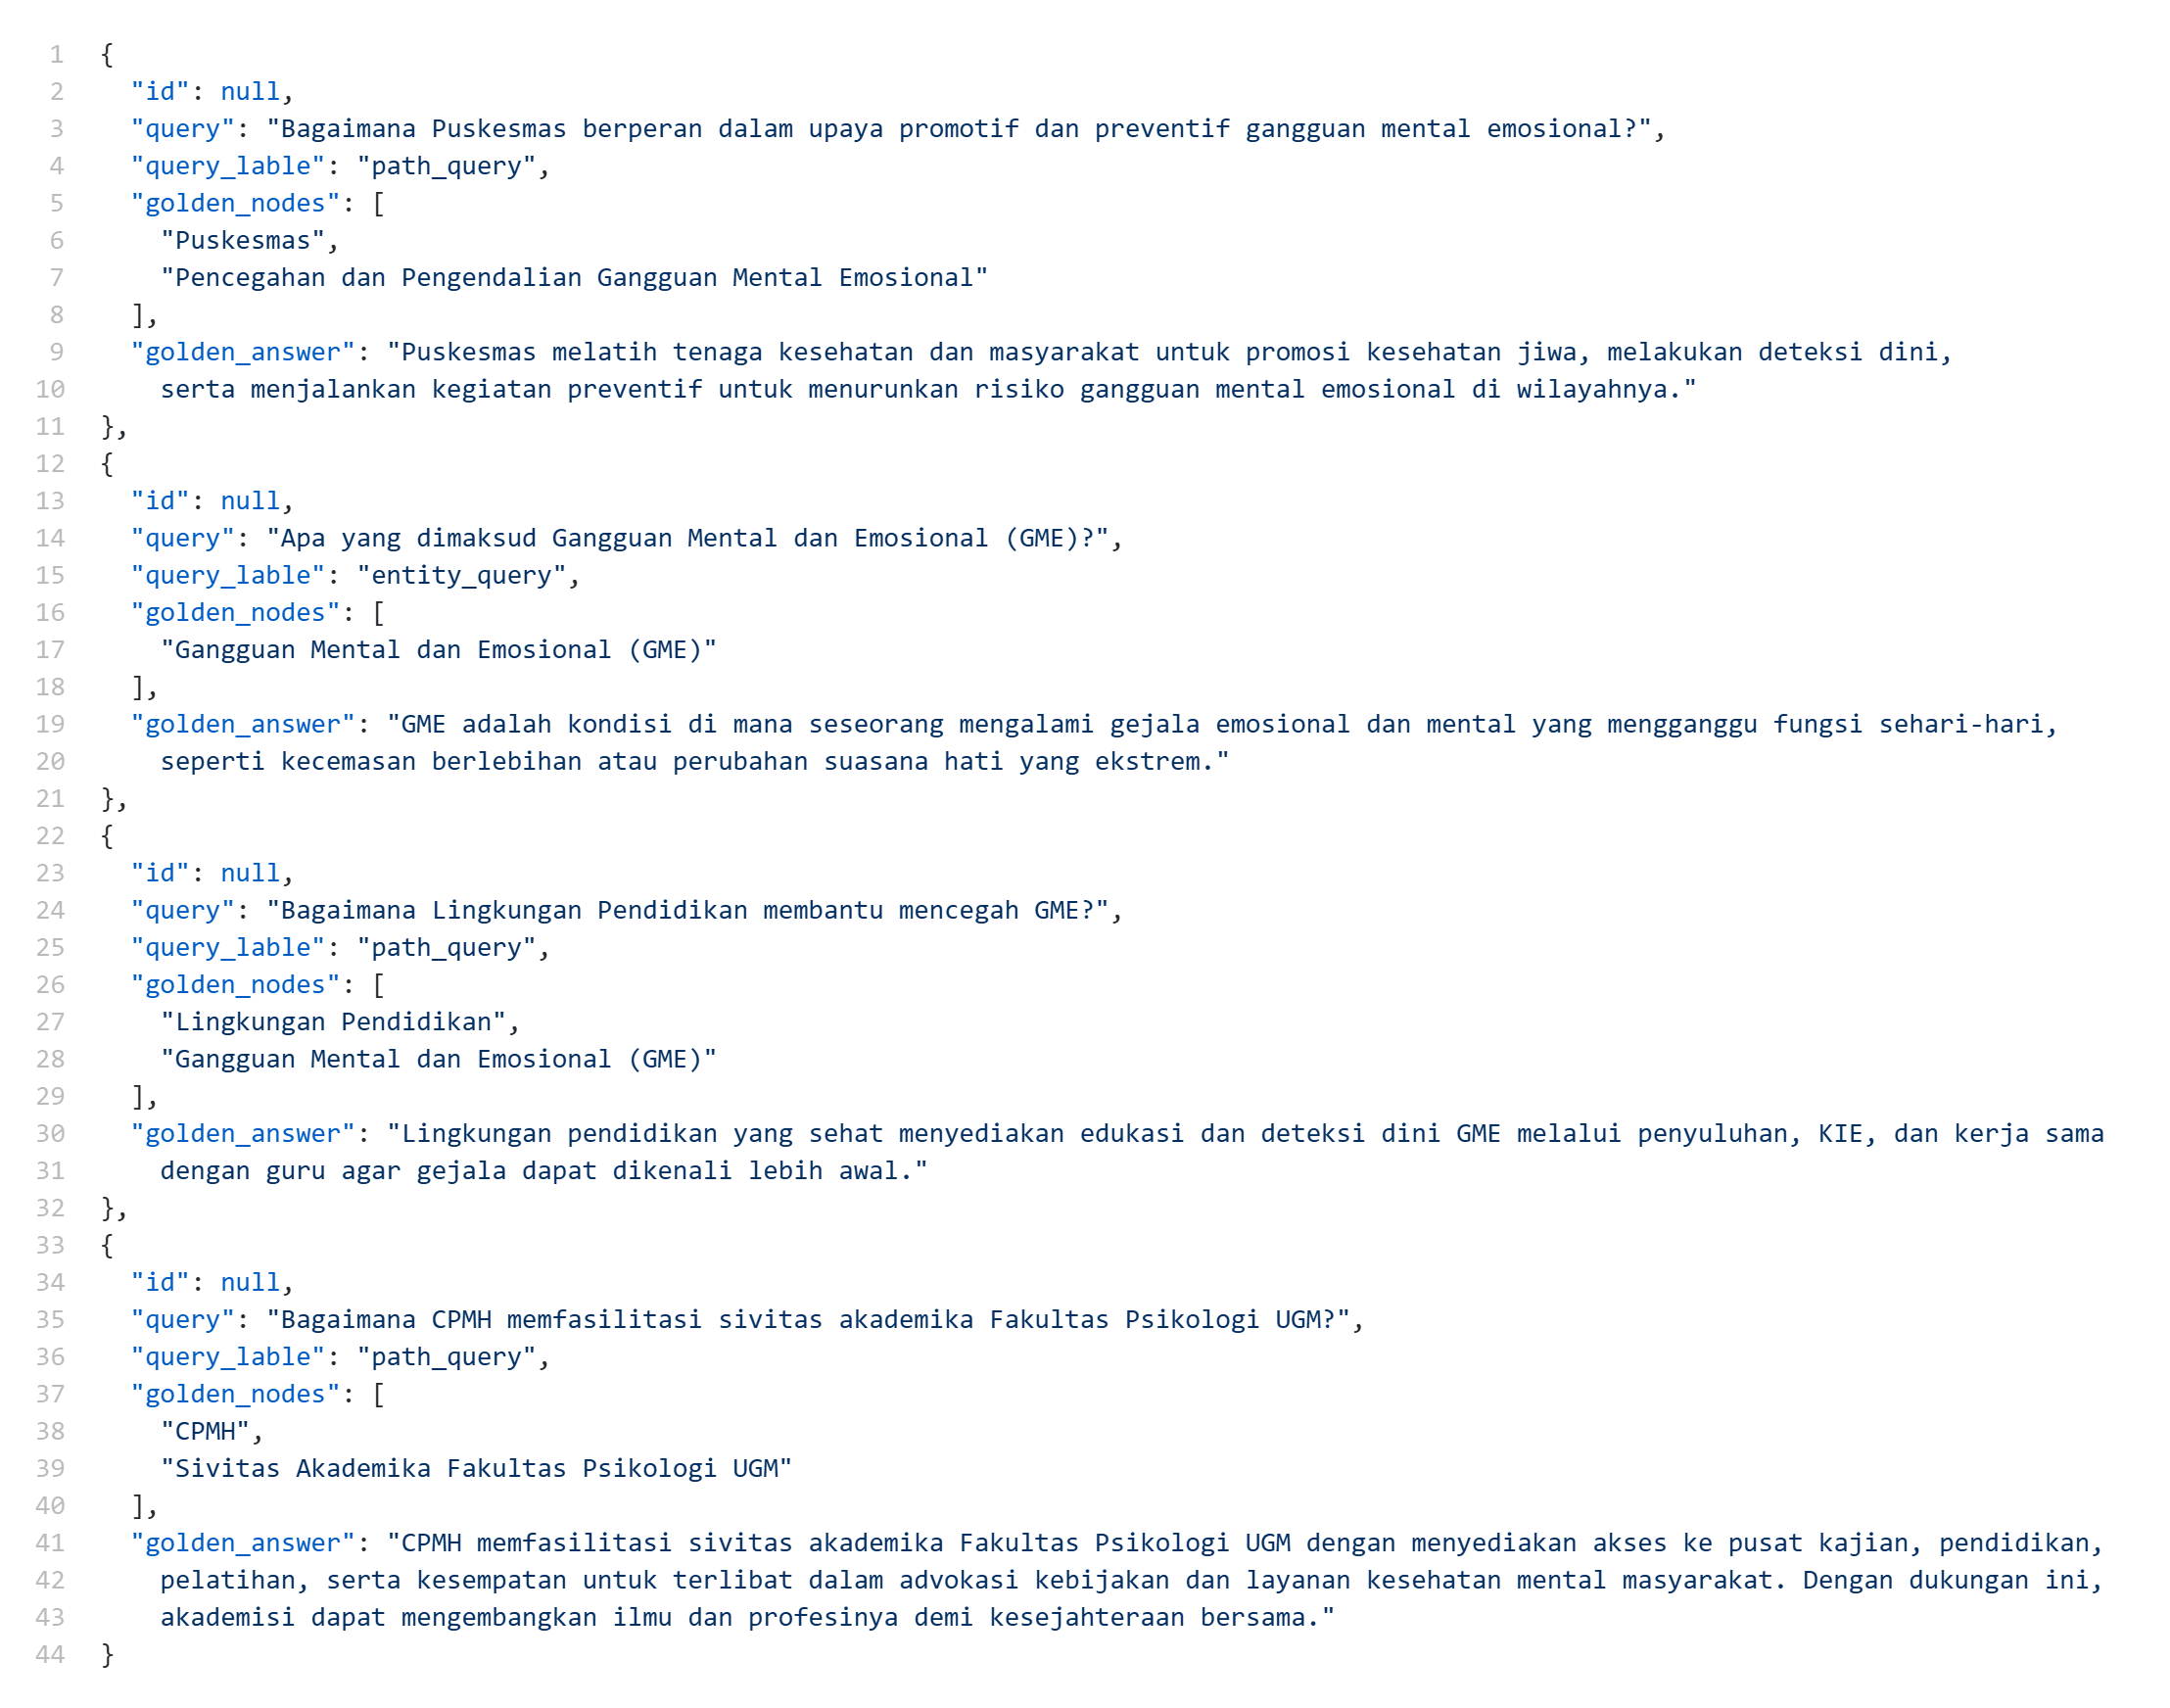
\includegraphics[width=\textwidth]{images/evaluation-dataset-example.png}}
	\caption{Contoh \textit{dataset} evaluasi sintesis yang dihasilkan oleh LLM}
	\label{fig:evaluation-dataset-example}
\end{figure}

Gambar \ref{fig:evaluation-dataset-example} menunjukkan contoh \textit{dataset} evaluasi yang mencakup kategori \\ \texttt{entity\_query} dan \texttt{path\_query}.
Setiap data sintetis terdiri dari 4 \textit{field} yaitu \textit{query}, \textit{query lable}, \textit{golden nodes}, dan \textit{golden answer}.
\textit{Query} merupakan pertanyaan yang jawabannya dapat diketahui dari informasi pada \textit{Knowledge Graph}.
Setiap kueri memiliki kategori yaitu \textit{entity query} atau \textit{path query} yang terdapat pada \textit{query lable}.
\textit{Golden nodes} berisi nodes yang diperlukan untuk menjawab pertanyaan pada \textit{field query}, sedangkan \textit{golden answer} merupakan jawaban yang dianggap benar untuk menjawab pertanyaan.

Pertanyaan \textit{"Apa yang dimaksud Gangguan Mental Emosional (GME)?"} termasuk ke dalam \texttt{entity\_query} karena menanyakan definisi dari suatu entitas yaitu Gangguan Mental Emosional (GME).
Jawaban dari pertanyaan tersebut seharusnya dapat ditemukan pada \textit{node} Gangguan Mental Emosional (GME) atau \textit{nodes} tetangganya.
\textit{Golden nodes} yang digunakan sebagai konteks untuk menjawab pertanyaan ini adalah Gangguan Mental Emosional (GME) sesuai dengan pertanyaan yang spesifik menanyakan GME.
\textit{Golden answer} yang dihasilkan secara langsung menjawab pertanyaan sesuai konteks yang diberikan yaitu dengan memberikan definisi dari GME.

Pada pertanyaan \textit{"Bagaimana CPMH memfasilitasi sivitas akademika Fakultas Psikologi UGM?"} terlihat ada dua entitas yang terkandung yaitu CPMH dan sivitas akademika Fakultas Psikologi.
Pertanyaan tersebut termasuk dalam \texttt{path\_query} karena jawabannya seharusnya dapat diperoleh dengan melihat hubungan antar entitas yang terkandung di dalamnya.
Untuk menjawab pertanyaan tersebut diperlukan dua \textit{nodes} yaitu CPMH dan Sivitas Akademika Fakultas Psikologi UGM seperti yang ada pada \textit{golden nodes} beserta \textit{nodes} lain yang berada di antara keduanya.
Jawaban yang terdapat pada \textit{golden answer} menjawab pertanyaan dengan memberikan hubungan antara CPMH dan sivitas akademika Fakultas Psikologi UGM yaitu sebagai fasilitator dilengkapi dengan contohnya.

\section{Analisis RAG Berbasis \textit{Knowledge Graph}}
Evaluasi sistem dilakukan pada dua keluaran utama RAG berbasis \textit{Knowledge Graph} yaitu konteks yang dikeluarkan oleh komponen \textit{retrieval} dan jawaban final yang dihasilkan.
Bagian \textit{retriever} dilakukan evaluasi untuk mengukur sejauh mana sistem dapat mengambil konteks yang relevan dari \textit{Knowledge Graph}.
Jawaban final akan diukur kualitas keluaran LLM setelah diberikan konteks dari \textit{retriever}.
Selain itu, dilakukan juga analisis kesalahan untuk mengidentifikasi penyebab kegagalan sistem dalam menjawab pertanyaan.

Evaluasi dilakukan dengan konfigurasi perlakuan seperti pada Tabel \ref{tab:evaluation-treatment} dengan mengatur parameter pada \textit{body} API.
Perlakuan dilakukan dengan mengatur dua parameter penentu algoritma yang digunakan oleh \textit{retriever} yaitu algoritma pencarian dan algoritma penelusuran graf.
Setiap pertanyaan pada \textit{dataset} evaluasi akan ditanyakan pada sistem dengan konfigurasi parameter menurut masing-masing perlakuan.
Naive RAG atau RAG berbasis potongan dokumen digunakan sebagai \textit{baseline} yang akan dibandingkan dengan RAG berbasis \textit{Knowledge Graph} terutama dalam hal kemampuannya menghasilkan jawaban final.

\begin{table}[H]
	\centering
	\caption{Perlakuan yang digunakan untuk mengevaluasi RAG berbasis \textit{Knowledge Graph} dengan \textit{naive} RAG sebagai \textit{baseline}}
	\label{tab:evaluation-treatment}
	\begin{tabular}{|l|p{9cm}|}
		\hline
		\textbf{Perlakuan}            & \textbf{Keterangan}                                                    \\
		\hline \hline
		\textbf{Naive RAG (Baseline)} &
		RAG dengan basis \textit{document chunk} menggunakan pencarian vektor sebagai \textit{retriever}.
		\textit{Document chunk} berukuran 1.200 karakter dengan overlap 400 karakter.
		Perlakuan ini digunakan sebagai \textit{baseline} evaluasi.                                            \\
		\hline
		\textbf{Default}              &
		\textit{Search method}: auto, \textit{graph traversal}: auto.

		Sistem otomatis memilih metode pencarian terbaik.
		Awalnya mencoba \textit{full-text search}, jika tidak ditemukan hasil, baru menggunakan pencarian vektor.
		Algoritma penelusuran graf ditentukan oleh modul klasifikasi kueri secara otomatis.                    \\
		\hline
		\textbf{Vector Search}        &
		\textit{Search method}: vector, \textit{graph traversal}: auto.

		Menggunakan pencarian node berbasis vektor (HNSW) dengan \textit{cosine similarity}.
		Algoritma penelusuran graf tetap otomatis.                                                             \\
		\hline
		\textbf{Neighbor Expansion}   &
		\textit{Search method}: auto, \textit{graph traversal}: neighbor\_expansion.

		Sistem menelusuri graf dengan algoritma \textit{one-hop neighbor expansion}, pencarian tetap otomatis. \\
		\hline
		\textbf{N-Shortest Path}      &
		\textit{Search method}: auto, \textit{graph traversal}: n-shortest\_path.

		Sistem menelusuri graf menggunakan algoritma \textit{n-shortest path}, pencarian tetap otomatis.       \\
		\hline
	\end{tabular}
\end{table}

Hasil dari \textit{request} pada sistem untuk setiap perlakuan pada Tabel \ref{tab:evaluation-treatment} menghasilkan data yang disimpan untuk evaluasi lebih lanjut.
Data hasil \textit{request} pada sistem yang disimpan terdiri atas \texttt{knowledge}, \texttt{llm\_answer}, \texttt{latency}, dan \texttt{graph\_entities}.
Komponen dari data tersebut yang kemudian akan dijadikan bahan evaluasi.
Latensi dari masing-masing perlakuan dapat dilihat pada Gambar \ref{fig:latency-per-treatment}

\begin{figure}[H]
	\centering
	\fbox{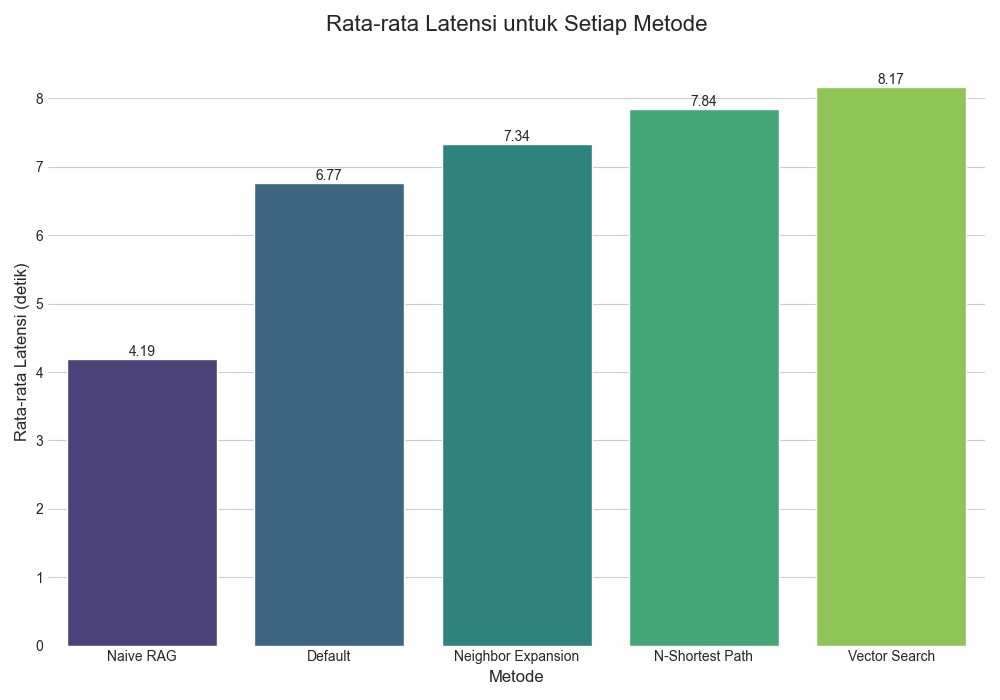
\includegraphics[width=0.8\textwidth]{images/grafik_perbandingan_latency.png}}
	\caption{Rerata latensi respons sistem pada setiap perlakuan}
	\label{fig:latency-per-treatment}
\end{figure}

Secara umum pendekatan Naive RAG memiliki rerata latensi yang lebih singkat yaitu 4,19 detik.
Angka ini lebih unggul dari RAG berbasis \textit{Knowledge Graph} yang memiliki latensi lebih dari 6 detik.
Hal tersebut dapat dipahami karena pada pendekatan berbasis \textit{Knowledge Graph} menggunakan pemanggilan LLM melalui API setidaknya sebanyak dua kali yaitu pada proses ekstraksi dan klasifikasi pada kueri serta pada tahap \textit{answer generation}.
Sebaliknya, Naive RAG hanya memerlukan satu kali pemanggilan LLM.
Selain itu komponen \textit{retriever} pada Naive RAG hanya perlu mencari dan mengambil potongan-potongan dokumen berdasarkan kemiripan teks, yang merupakan operasi yang lebih cepat dan tidak memerlukan proses penelusuran kompleks.

\textit{Knowledge} atau konteks yang dihasilkan oleh komponen \textit{retriever} akan dipakai sebagai konteks tambahan bagi LLM untuk menjawab pertanyaan.
Rerata panjang konteks dari masing-masing perlakukan dapat dilihat pada Gambar \ref{fig:context-length-per-treatment}.

\begin{figure}[H]
	\centering
	\fbox{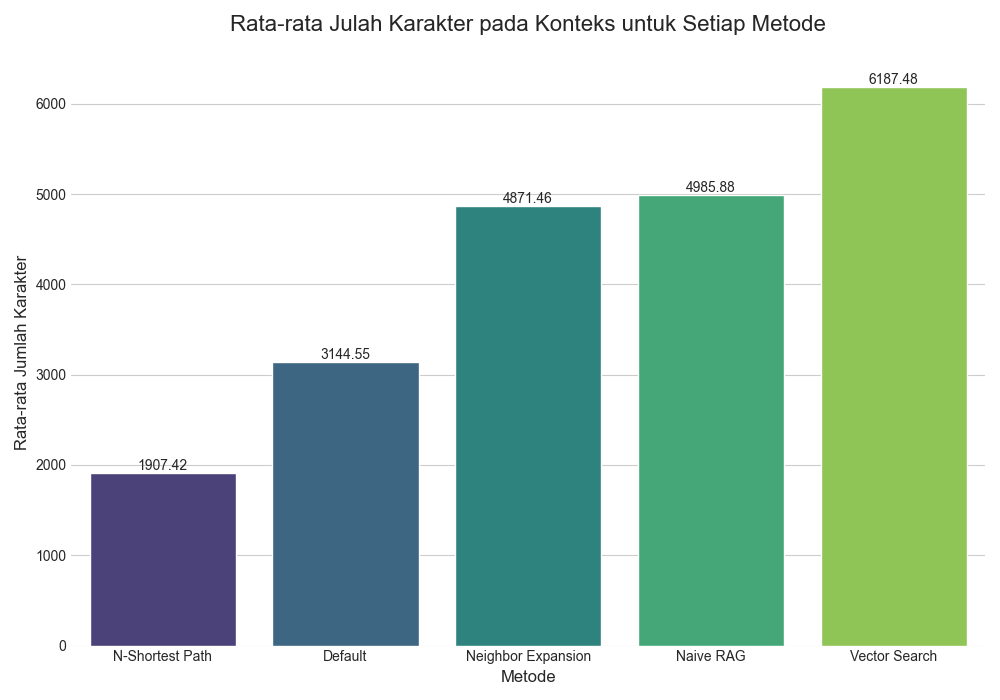
\includegraphics[width=0.8\textwidth]{images/grafik_perbandingan_konteks.png}}
	\caption{Rerata panjang konteks dari respons sistem pada setiap perlakuan}
	\label{fig:context-length-per-treatment}
\end{figure}

Dari Gambar \ref{fig:context-length-per-treatment} dapat dilihat pendekatan berbasis \textit{Knowledge Graph} secara umum memiliki panjang konteks yang lebih sedikit dari Naive RAG kecuali pada Vector Search.
Pendekatan N-Shortest Path menghasilkan rerata panjang konteks paling sedikit sebanyak 1907,42 kemudian diikuti oleh Default (3144,55), Neighbor Expansion (4871,46), Naive RAG (4985,88), dan Ventor Search (6187,48).
Hal tersebut dapat dipahami karena pendekatan dengan pencarian jalur menghasilkan lebih sedikit entitas dibandingkan dengan pendekatan ekspansi tetangga.
Pendekatan Default terlihat sebagai titik tengah antara N-Shortest Path dan Neighbor Expansion karena secara dinamis menentukan algoritma penelusuran graf yang sesuai.
Pendekatan berbasis vektor seperti pada Naive RAG dan Vector Search cenderung menghasilkan konteks yang lebih panjang karena menggunakan $k$ dokumen atau \textit{node} teratas berdasarkan kemiripan (dengan $k=5$ dalam kasus ini) yang secara inheren cenderung menarik lebih banyak teks dibandingkan pencarian dengan \textit{full-text search}.

Konteks yang lebih panjang secara intuitif akan membuat LLM memerlukan waktu pemrosesan lebih lama yang akan memengaruhi latensi respons sistem secara keseluruhan.
Hal tersebut dapat dilihat pada Gambar \ref{fig:context-length-vs-latency} yang menunjukkan adanya hubungan positif.
Semakin banyak konteks yang diberikan pada LLM akan menghasilkan latensi respons yang lebih lama.

\begin{figure}[H]
	\centering
	\fbox{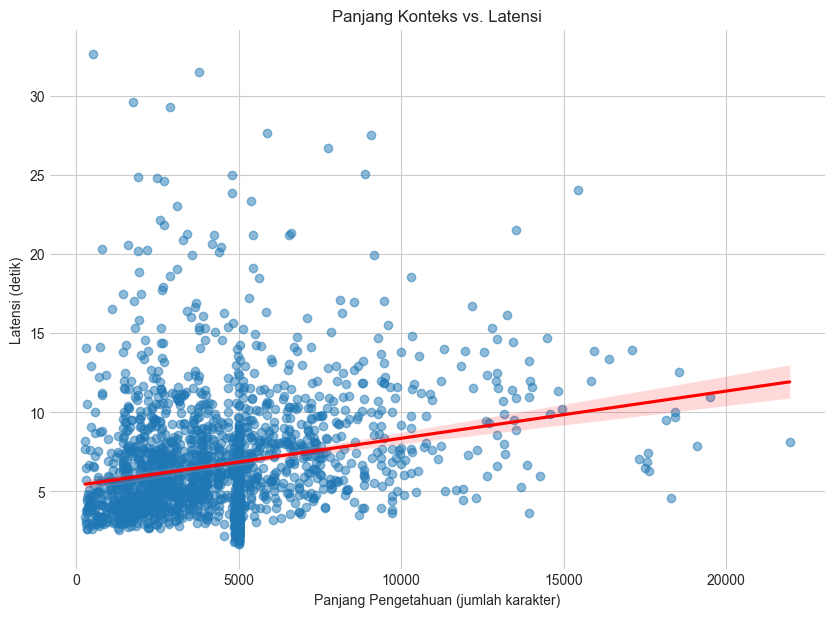
\includegraphics[width=0.8\textwidth]{images/panjag_konteks_vs_latensi.png}}
	\caption{\textit{Scatter plot} panjang konteks dengan latensi keseluruhan respons}
	\label{fig:context-length-vs-latency}
\end{figure}
\subsection{Analisis Kinerja Komponen \textit{Retriever}}

Pengujian komponen \textit{retriever} dilakukan untuk mengukur kualitas informasi atau konteks yang diambil dari \textit{Knowledge Graph}.
Informasi yang terdapat pada \textit{Knowledge Graph} berupa kumpulan \textit{nodes} yang dihubungkan oleh \textit{vertex} tertentu.
Alih-alih mengevaluasi konteks yang sudah berupa teks panjang yang memerlukan alat seperti LLM yang kurang pasti dalam menguji, pengujian dilakukan pada \textit{nodes} yang dihasilkan sehingga evaluasi lebih terkontrol dan akurat.
Terdapat empat metrik uji untuk mengevaluasi kinerja komponen \textit{retriever} yaitu \textit{precision}, \textit{recall}, \textit{Mean Reciprocal Rank} (MRR), dan \textit{hit ratio}.
Tabel \ref{tab:retrieval-evaluation-result} menunjukkan hasil pengujian empat metrik uji tersebut terhadap empat perlakukan pada Tabel \ref{tab:evaluation-treatment}.

\begin{table}[H]
	\centering
	\caption{Hasil evaluasi \textit{retriever} pada RAG berbasis \textit{Knowledge Graph} untuk masing-masing perlakuan}
	\label{tab:retrieval-evaluation-result}
	\begin{tabular}{|l|c|c|c|c|}
		\hline
		\textbf{Perlakuan}          & \textbf{Precision} & \textbf{Recall} & \textbf{MRR} & \textbf{Hit Ratio} \\
		\hline \hline
		\textbf{Default}            & 0,1530             & 0,8203          & 0,3758       & 0,9053             \\
		\hline
		\textbf{Vector Search}      & 0,0603             & 0,5929          & 0,1737       & 0,6744             \\
		\hline
		\textbf{Neighbor Expansion} & 0,1123             & 0,8868          & 0,3191       & 0,9584             \\
		\hline
		\textbf{N-Shortest Path}    & 0,1245             & 0,5370          & 0,2788       & 0,6097             \\
		\hline
	\end{tabular}
\end{table}

Berdasarkan hasil pada Tabel \ref{tab:retrieval-evaluation-result}, terlihat bahwa nilai \textit{precision} tertinggi dicapai oleh perlakuan Default (0,1530), yang menunjukkan bahwa metode ini mampu menghasilkan proporsi konteks relevan tertinggi dibandingkan dengan total konteks yang diambil.
Sebaliknya, metode Vector Search memiliki \textit{precision} terendah (0,0603), mengindikasikan banyaknya informasi yang tidak relevan diambil.
Pada metrik \textit{Recall}, nilai tertinggi diperoleh oleh Neighbor Expansion (0,8868), yang berarti metode ini paling mampu mengambil informasi relevan sebanyak mungkin dari \textit{Knowledge Graph}.
Namun, metode N-Shortest Path mencatat nilai \textit{recall} terendah (0,5370), menandakan adanya keterbatasan dalam menjangkau konteks relevan.

Metrik \textit{Mean Reciprocal Rank} tertinggi juga dicapai oleh Default (0,3758), mengindikasikan bahwa konteks relevan cenderung berada pada urutan teratas hasil pencarian.
Sebaliknya, Vector Search menempati posisi terendah (0,1737) yang mengindikasikan konteks relevan sering berada pada urutan bawah.
Untuk \textit{Hit Ratio}, nilai tertinggi kembali diraih oleh Neighbor Expansion (0,9584), menandakan bahwa metode ini hampir selalu berhasil menemukan setidaknya satu konteks relevan dalam hasil pencarian.
Sebaliknya, N-Shortest Path mencatat \textit{hit ratio} terendah (0,6097), menunjukkan probabilitas yang lebih rendah untuk menemukan konteks relevan pada setiap kueri.

Dari keempat metrik, terlihat adanya \textit{trade-off} antara \textit{precision} dan \textit{recall}.
Metode Default unggul pada \textit{precision} dan MRR, namun \textit{recall}-nya lebih rendah dibandingkan Neighbor Expansion.
Hal ini mengindikasikan bahwa Default lebih selektif dalam mengambil konteks, sedangkan Neighbor Expansion lebih agresif dan luas cakupannya, sehingga \textit{recall}-nya tinggi tetapi precision-nya moderat.
Vector Search cenderung kurang optimal di semua metrik, menunjukkan bahwa pendekatan berbasis vektor saja kurang efektif jika tidak dipadukan dengan strategi traversal pada \textit{Knowledge Graph}.
Sementara itu, N-Shortest Path memberikan hasil yang seimbang namun tidak menonjol pada metrik \textit{precision}, tetapi kurang optimal untuk metrik lainnya.
Secara keseluruhan, Neighbor Expansion menjadi metode yang paling konsisten untuk memaksimalkan jangkauan informasi (\textit{recall} dan \textit{hit ratio} tinggi), sedangkan Default unggul dalam mempertahankan relevansi pada hasil teratas (\textit{precision} dan MRR tinggi).

\subsection{Analisis Respons Final}
Pengujian respons final dilakukan untuk mengukur kualitas jawaban akhir yang dihasilkan oleh RAG berbasis \textit{Knowledge Graph} setelah diberikan konteks tambahan oleh komponen \textit{retriever}.
Informasi berupa subgraf yang terdiri dari kumpulan \textit{nodes} dan \textit{edges} yang terhubung ditransformasikan ke dalam bentuk tekstual yang lebih makna semantik.
Bentuk tekstual tersebut kemudian dijadikan sebagai konteks untuk memberikan informasi tambahan dalam menghasilkan jawaban.
Jawaban akhir dievaluasi dengan memperhatikan empat parameter yaitu pertanyaan, jawaban yang dihasilkan, konteks, dan jawaban seharusnya sebagai \textit{ground truth}.

Evaluasi dilakukan dengan pustaka \textit{framework} RAGAS (Retrieval-Augmented Generation Assessment) yang merupakan evaluator RAG dengan salah satu alat ujinya menggunakan LLM.
Metrik uji untuk mengevaluasi jawaban adalah \textit{similarity}, \textit{correctness}, \textit{relevancy}, dan \textit{faithfulness} yang merupakan metrik bawaan RAGAS.
Tabel \ref{tab:final-answer-evaluation-result} menunjukkan hasil evaluasi RAGAS pada masing-masing perlakukan termasuk dengan \textit{baseline Naive} RAG.

\begin{table}[H]
	\centering
	\caption{Hasil evaluasi jawaban final pada RAG berbasis \textit{Knowledge Graph} untuk masing-masing perlakuan dan dibandingkan dengan \textit{baseline naive} RAG}
	\label{tab:final-answer-evaluation-result}
	\begin{tabular}{|l|c|c|c|c|}
		\hline
		\textbf{Perlakuan}          & \textbf{Similarity} & \textbf{Correctness} & \textbf{Relevancy} & \textbf{Faithfulness} \\
		\hline \hline
		\textbf{Naive RAG}          & 0,9048              & 0,3391               & 0,6996             & 0,8993                \\
		\hline
		\textbf{Default}            & 0,9242              & 0,4155               & 0,8624             & 0,9435                \\
		\hline
		\textbf{Vector Search}      & 0,9115              & 0,3895               & 0,7387             & 0,8902                \\
		\hline
		\textbf{Neighbor Expansion} & 0,9248              & 0,4246               & 0,8723             & 0,9428                \\
		\hline
		\textbf{N-Shortest Path}    & 0,9033              & 0,3936               & 0,7900             & 0,4614                \\
		\hline
	\end{tabular}
\end{table}

Metrik \textit{similarity} mengukur kesamaan semantik dengan membandingkan bentuk vektor (\textit{embedding}) antara jawaban yang dihasilkan sistem dan jawaban \textit{ground truth}.
Hasil menunjukkan bahwa semua perlakuan, termasuk \textit{baseline} Naive RAG, memiliki skor \textit{similarity} yang relatif tinggi di atas 0,9, menandakan bahwa sistem mampu menghasilkan jawaban yang secara umum memiliki kedekatan makna dengan jawaban seharusnya.
Nilai tertinggi dicapai oleh perlakuan Neighbor Expansion (0,9248) dan Default (0,9242), yang mengindikasikan bahwa perluasan konteks berbasis \textit{Knowledge Graph} secara umum sama efektifnya dalam menjaga kesamaan makna dibandingkan dengan \textit{baseline}.

Metrik \textit{correctness} menilai kebenaran faktual dari jawaban yang dihasilkan.
Hasil menunjukkan peningkatan hingga sebesar 8,55\% pada perlakuan yang memanfaatkan \textit{Knowledge Graph} traversal khususnya pada perlakikan Neighbor Expansion (0,4246) dan  Default (0,4155) dibanding \textit{baseline} Naive RAG (0.3391).
Hal ini mengindikasikan bahwa penelusuran graf yang tepat dapat membantu sistem menemukan konteks yang lebih faktual.

Relevansi menunjukkan sejauh mana jawaban sesuai dengan pertanyaan yang diajukan.
Neighbor Expansion (0,8723) dan Default (0,8624) lebih unggul sekitar 17\% dari Naive RAG (0,6996) pada metrik ini.
Peningkatan tersebut menunjukkan bahwa konteks yang dihasilkan dari \textit{Knowledge Graph} tidak hanya  jawaban lebih faktual, tetapi juga lebih tepat sasaran.
Konteks yang lebih tepat sasaran akan membuat jawaban yang dihasilkan lebih relevan dengan pertanyaan.

\textit{Faithfulness} mengukur kesesuaian informasi dalam jawaban dengan konteks yang diberikan.
Hampir semua metode memiliki nilai di atas 0,89, kecuali N-Shortest Path yang sangat rendah (0,4614), menandakan bahwa metode ini sering menghasilkan jawaban yang tidak konsisten atau tidak sepenuhnya didukung oleh konteks.
Nilai tinggi pada Default (0,9435) dan Neighbor Expansion (0,9428) menunjukkan bahwa strategi ini paling konsisten dalam menggunakan informasi yang tersedia.
RAG \textit{Knowledge Graph} dengan strategi tersebut tetap lebih tinggi sekitar 4\% dibandingkan dengan \textit{baseline} Naive RAG menghasilkan skor (0,8993).
Ini adalah bukti bahwa konteks yang diperkaya oleh \textit{Knowledge Graph} secara efektif mengurangi LLM dari halusinasi atau mengarang informasi.

Hasil evaluasi jawaban final secara umum menunjukkan bahwa penggunaan \textit{Knowledge Graph} yang tepat dapat meningkatkan kualitas jawaban akhir secara signifikan.
Neighbor Expansion menjadi strategi terbaik karena konsisten unggul di semua metrik kecuali \textit{faithfulness}, yang tetap sangat tinggi.
Perlakuan Default juga menjadi alternatif yang andal dengan kinerja mendekati Neighbor Expansion tanpa konfigurasi khusus.
Penggunaan metode pencarian Vector Search secara langsung tidak mampu mengungguli metode pencarian dengan \textit{full-text} dalam hal relevansi dan \textit{correctness}.
Sementara itu, penggunaan N-Shortest Path dalam melakukan penelusuran graf secara umum berpotensi menghasilkan jawaban yang tidak optimal ditandai dengan skor \textit{faithfulness} yang sangat rendah bahkan lebih rendah dibandingkan dengan \textit{baseline}.

\subsection{Analisis Kesalahan dan Studi Kasus}

Analisis terakhir adalah meninjau secara langsung jawaban yang di hasilkan oleh masing-masing metode.
Pada studi kasus kueri \textit{"Apa yang dimaksud dengan gejala psikotik?"}, terlihat perbedaan kualitas jawaban yang dihasilkan oleh berbagai metode RAG berbasis \textit{Knowledge Graph}.
Jawaban yang diharapkan (\textit{golden answer}) memuat penjelasan singkat bahwa gejala psikotik meliputi halusinasi atau delusi seperti mendengar suara, yang dapat memengaruhi pola pikir dan berisiko terkait pikiran bunuh diri.
Hasil jawaban secara lengkap dapat dilihat pada Tabel \ref{tab:final-answer-case-1}.

\begin{longtable}{|p{2cm}|p{11cm}|}
	\caption{Komparasi kueri dan jawaban oleh masing-masing metode} \label{tab:final-answer-case-1}                                                                                                                                                                                                                                \\
	\hline
	\textbf{Kueri}                  & Apa yang dimaksud dengan gejala psikotik?                                                                                                                                                                                                                                                    \\
	\hline \hline

	\textbf{Golden Answer}          & Gejala psikotik meliputi halusinasi atau delusi seperti mendengar suara yang dapat memengaruhi cara seseorang berpikir dan berisiko terkait pikiran bunuh diri. (\textbf{Terdapat Konteks})                                                                                                  \\
	\hline
	\textbf{Naive RAG}              & Mohon maaf, konteks yang diberikan tidak menjelaskan apa yang dimaksud dengan gejala psikotik. Konteks tersebut hanya menyebutkan tentang individu risiko tinggi psikotik dan pencegahan transisi menjadi gangguan psikotik. (\textbf{Terdapat Konteks})                                     \\
	\hline
	\textbf{Default}                & Gejala psikotik adalah gejala yang mungkin dialami oleh Orang dengan Kebutuhan Disabilitas (OKBD) yang bisa memengaruhi keinginan bunuh diri, contohnya adalah mendengar suara-suara. (\textbf{Terdapat Konteks})                                                                            \\
	\hline
	\textbf{Vector \newline Search} & Saya mohon maaf, saya tidak menemukan informasi spesifik mengenai "gejala psikotik" dalam pengetahuan yang saya miliki. Pengetahuan yang tersedia lebih berfokus pada keluhan fisik, gejala somatik, faktor biologis, dan tanda bahaya kecenderungan bunuh diri. (\textbf{Terdapat Konteks}) \\
	\hline
	\textbf{Neighbor Expansion}     & Gejala psikotik adalah gejala yang mungkin dialami oleh Orang dengan Kondisi Biologis dan Diagnosa (OKBD) yang bisa memengaruhi keinginan bunuh diri, seperti mendengar suara-suara. Gejala ini juga dapat memperbesar risiko bunuh diri. (\textbf{Terdapat Konteks})                        \\
	\hline
	\textbf{N-Shortest Path}        &
	\begin{minipage}[t]{10cm}
		Gejala psikotik adalah serangkaian pengalaman yang menunjukkan hilangnya kontak dengan realitas. Ini sering kali melibatkan perubahan dalam pikiran, persepsi, dan perilaku seseorang.

		Gejala psikotik utama meliputi:
		\begin{enumerate}
			\item \textbf{Halusinasi:} Persepsi sensorik tanpa rangsangan eksternal.
			\item \textbf{Delusi:} Keyakinan salah yang bertahan meskipun ada bukti bertentangan.
			\item \textbf{Pemikiran dan Bicara Tidak Terorganisir:} Kesulitan mengatur pikiran sehingga bicara menjadi kacau.
			\item \textbf{Perilaku Tidak Terorganisir atau Katatonik:} Perilaku aneh, agitasi, atau tidak bergerak sama sekali.
		\end{enumerate}
		(\textbf{Tanpa Konteks})
		\vspace{0.5em}
	\end{minipage}                                                                                                                                          \\
	\hline
\end{longtable}

Metode Naive RAG gagal memberikan definisi langsung, hanya menyampaikan bahwa konteks tidak menjelaskan gejala psikotik dan sekadar menyinggung individu berisiko tinggi psikotik serta pencegahan transisi menjadi gangguan psikotik.
Jawaban tersebut menunjukkan bahwa meskipun \textit{retriever} memberikan konteks, isi dari konteks tersebut belum tentu relevan dan sesuai untuk menjawab pertanyaan.
Untuk pertanyaan yang spesifik menyebutkan suatu istilah atau pun menanyakan definisi mengenai suatu hal, pencarian menggunakan vektor terkadang kesulitan untuk menghasilkan hasil yang dimaksud.
Hal serupa juga dapat dilihat pada strategi Vector Search pada \textit{Knowledge Graph}.
Vector Search menunjukkan jawaban yang mengaku tidak menemukan informasi spesifik dan malah memaparkan topik terkait keluhan fisik, faktor biologis, dan tanda bahaya kecenderungan bunuh diri, yang hanya sedikit relevan dengan kueri.
Hal tersebut mengindikasikan representasi vektor dari data terkadang mengalami kesulitan untuk menangkap makna semantik dari kueri yang berbentuk definisi singkat atau mengandung istilah khusus.

Sebaliknya, Default dan Neighbor Expansion berhasil mendekati topik yang benar, menyebutkan bahwa gejala psikotik dapat memengaruhi keinginan bunuh diri dan memberikan contoh seperti mendengar suara-suara.
Namun, kedua metode ini cenderung menggunakan istilah "OKBD" atau "Orang dengan Kondisi Biologis dan Diagnosa" yang tidak disebutkan dalam jawaban seharusnya, sehingga relevansi dan kesesuaian makna hanya sebagian terpenuhi.

Di sisi lain Metode N-Shortest Path menghasilkan jawaban yang secara definisi umum sangat lengkap dan mencakup empat gejala utama (halusinasi, delusi, pemikiran/bicara tidak terorganisir, dan perilaku tidak terorganisir atau katatonik).
Meskipun tampak informatif, jawaban ini merupakan bentuk halusinasi karena tidak bersumber dari konteks yang diambil oleh \textit{retriever}.
\textit{Retriever} gagal untuk mengambil konteks dari \textit{Knowledge Graph} yang menyebabkan LLM memanfaatkan pengetahuan internalnya untuk mengisi kekosongan informasi.
Kegagalan tersebut dapat dipicu oleh algoritma \textit{shortest path} di mana tidak ditemukannya jalur di antara \textit{nodes} yang terdeteksi.
Hal tersebut dapat terjadi apa bila memaksakan pertanyaan yang termasuk ke dalam \textit{entity query} dalam kasus ini \textit{"Apa yang dimaksud dengan gejala psikotik?"} yang menanyakan definisi akan suatu hal.

Dari kasus ini dapat disimpulkan bahwa kelengkapan jawaban tidak selalu berarti kualitas RAG yang baik.
Metode yang terlihat "pintar" seperti N-Shortest Path bisa saja menyalurkan halusinasi jika \textit{retrieval} tidak relevan.
Sebaliknya, metode seperti Default dan Neighbor Expansion yang memanfaatkan konteks dengan benar cenderung lebih \textit{faithful}, walau informasi yang dihasilkan mungkin lebih terbatas.
Temuan ini memperkuat pentingnya mengukur metrik seperti \textit{faithfulness} secara terpisah dari \textit{similarity}, karena keduanya bisa menunjukkan arah evaluasi yang berbeda.


% Berikut ini adalah yang perlu diperhatikan untuk mengisi bab hasil dan pembahasan:

% \begin{enumerate}
% 	\item Setiap rumusan masalah boleh memiliki lebih dari 1 tujuan.
% 	\item Setiap subbab harus spesifik menjawab setiap tujuan yang dituliskan.
% 	\item Setiap rumusan masalah boleh dijawab dengan 1 subbab atau lebih.
% \end{enumerate}

% Berikut ini adalah contoh sub bab untuk menjelaskan tujuan penelitian.

% \section{Pembahasan Tujuan 1 dengan Hasil Penelitian 1 (Ubah Judul Sesuai dengan Hal yang Hendak dibahas)}

% Sub bab pertama adalah membahas tujuan penelitian pertama dengan hasil penelitian ke-1.
% Dapat ditambahkan beberapa sub bab jika diperlukan.

% \section{Pembahasan Tujuan 1 dengan Hasil Penelitian 2 (Ubah Judul Sesuai dengan Hal yang Hendak dibahas)}

% Sub bab kedua adalah membahas tujuan penelitian pertama dengan hasil penelitian ke-2. Sub bab ini merupakan contoh tambahan sub bab pertama.

% \section{Pembahasan Tujuan 2 dengan Hasil Penelitian 3 (Ubah Judul Sesuai dengan Hal yang Hendak dibahas)}

% Sub bab ketiga adalah membahas tujuan penelitian kedua. Dapat ditambahkan beberapa sub bab jika diperlukan.

% \section{Perbandingan Hasil Penelitian dengan Hasil Terdahulu}

% Pembahasan penutup dapat menjelaskan mengenai kelebihan hasil pengembangan /
% penelitian dan kekurangan dibandingkan dengan skripsi atau penelitian terdahulu atau
% perbandingan terhadap produk lain yang ada di pasaran. Penulis dapat menggunakan tabel untuk membandingkan secara gamblang dan menjelaskannya.